\section{Estimating continuous-valued neural representational geometry with denoising score matching}

\subsection{Introduction}
Representational similarity analysis is widely used in neuroscience and cognitive science to characterize how neural populations encode stimuli by estimating a representational dissimilarity matrix. Existing approaches have provided useful tools for this purpose, including correlation-based distances, Euclidean distances. However, these methods does not account for the noise structure of the data, and is variant to subjective choices of the coordinate system. Mahalanobis distances and decoding-based measures exploit the statistical nature of the problem. However, in order to estimate covariance or decoding, data must be binned first. Binning breaks the continuous nature of the problem, furthermore, when the number of data is sparse, binning reduce the number of data points even more, reducing the method reliability. Other methods like Wishart process does not binning the data yet requires explicitly assume the statistical model of the data (e.g. simple Gaussian) which is often to simplistic.

Here we propose a score-based continuous-stimulus method for estimating representational geometry directly from neural responses without binning the stimulus variable. Our method exploits the smooth structure of the stimulus axis by estimating the conditional score of the neural response distribution with respect to stimulus using score matching (a type of diffusion model), and then using this quantity to construct pairwise dissimilarities with a direct probabilistic interpretation. This provides a principled framework for recovering representational geometry of continuous-valued stimuli from sparse and noisy neural data.

\subsection{Methods}
Denoting the continuous-valued stimulus variable as $\theta$, and the neural population response is modeled as a conditional distribution $p(x\mid \theta)$ which is unknown. A dataset is sampled from the joint distribution $p(x, \theta) = p(\theta)p(x\mid \theta)$ where $p(\theta)$ is the prior distribution which is often known by the experimenter (e.g. sampling uniform orientation of the grating image) or easy to estimate because of the low-dimensional nature of the stimulus.

Representation dissimilarity analysis cares about the "distance" between two stimulus conditions, mathematically, the distance between two conditional distributions. A straightforward choice is KL divergence, however, KL divergence is not a real distance metric. Therefore in this project, we use Hellinger distance $H(p_i,p_j)$
\[
H^2(p_i,p_j)
=
1-\int \sqrt{p(x\mid \theta_i)\,p(x\mid \theta_j)}\,dx,
\qquad
p_i:=p(x\mid \theta_i),\;\; p_j:=p(x\mid \theta_j).
\]
Besides being a true distance metric, Hellinger distance is attractive here for two additional reasons. First, it is locally connected to Fisher information. When two stimulus conditions are infinitesimally close, the squared Hellinger distance reduces, to leading order, to the Fisher-information metric. Second, Hellinger distance bounds the performance of the optimal binary classifier. In particular, a larger Hellinger distance implies a smaller achievable Bayes error. For these reasons, Hellinger distance provides a natural probabilistic notion of representational dissimilarity.

To connect Hellinger distance to a quantity that can be estimated from samples, define the log-likelihood ratio
\[
\Delta \ell_{ij}(x)
:=
\log p(x\mid \theta_j)-\log p(x\mid \theta_i).
\]
Then the Bhattacharyya affinity can be written as
\[
\sqrt{p(x\mid \theta_i)\,p(x\mid \theta_j)}
=
p(x\mid \theta_i)\exp\!\left(\frac{\Delta \ell_{ij}(x)}{2}\right),
\]
which yields
\[
H^2(p_i,p_j)
=
1-
\mathbb E_{x\sim p_i}
\left[
\exp\!\left(\frac{\Delta \ell_{ij}(x)}{2}\right)
\right].
\]
Although exact, this one-sided form is asymmetric at the sample level because the expectation is taken only under \(p_i\). To obtain a symmetric sample-wise quantity, we instead use the identity
\[
H^2(p_i,p_j)
=
\frac12\,
\mathbb E_{x_i\sim p_i,\;x_j\sim p_j}
\left[
h_{ij}(x_i)+h_{ij}(x_j)
\right],
\]
where
\[
h_{ij}(x)
:=
1-\operatorname{sech}\!\left(\frac{\Delta \ell_{ij}(x)}{2}\right).
\]
This form is explicitly symmetric in \(i\) and \(j\), and expresses the Hellinger distance as the average of two sample-wise contributions, one evaluated on \(x_i\sim p_i\) and the other on \(x_j\sim p_j\).

The remaining challenge is therefore to estimate \(\Delta \ell_{ij}(x)\) without discretizing \(\theta\). To exploit the continuous nature of the problem, we decompose the log-likelihood ratio into integration
\[
\Delta \ell_{ij}(x)
=
\int_{\theta_i}^{\theta_j}
\partial_\theta \log p(x\mid \theta)\,d\theta.
\]
If we are able to estimate the Fisher score of all data points $\theta_i$, integration can be computed numerically into summation.

How to estimate Fisher score? We use Bayes' rule:
\[
\partial_\theta \log p(x\mid \theta)
=
\partial_\theta \log p(\theta\mid x)-\partial_\theta \log p(\theta).
\]
The gradient of prior distribution can be computed analytically if the prior distribution is known by the experimentalist; if not known, estimating is relatively straightforward due to the low-dimensional nature of the stimulus.

We use denoising score matching to estimate $\partial_\theta \log p(\theta\mid x)$. The detail is written in previous section.

Overall, the pipeline is the following: Given a dataset $\{(\theta_i,x_i)\}_{i=1}^N$, we estimate the Fisher score of all data points $\theta_i$ using denoising score matching, and then perform path integration to obtain log-likelihood ratio, finally compute $h_{ij}(x)$. Notably, there's no data binning in this pipline. The final $H_{ij}$ is the expecation of $h_{ij}(x)$ over all data points $x_i$ and $x_j$, which can be estimated by simple binning, or more consistently using Gaussian process regression to estimate without any binning. But for simplicity, we use binning in preliminary results. The details of the pipeline is given in Supplementary Information.

\subsection{Preliminary results}

We generated a toy 2D linear model where neural tuning is $(x, 2x)$ with independent Gaussian noise std linearly ramped from 0.2 to 4. As an approximation of the ground truth, we generate large dataset with 5000 sample points and then estimated Hellinger distance matrix and pairwise decoding matrix, respectively. Hellinger distance matrix is estimated as stated in the method section; pairwise decoding matrix is estimated by binning the data and use logistic regression.

To study how well each of these two methods performs when the dataset size is small, we subsampled smaller dataset with $n = 50, $ sample points. For each of the subsampled dataset, we estimated RDM respectively and then compared the correlation of the off-diagonal entries to the approximated ground truth RDM.

Results showing that our Hellinger distance matrix estimated by denoising score matching method exploit the continuous nature of the problem and converges faster than pairwise decoding method, see Figure~\ref{fig:rsa_nested_subset_convergence}.


\begin{figure}[htbp]
    \centering
    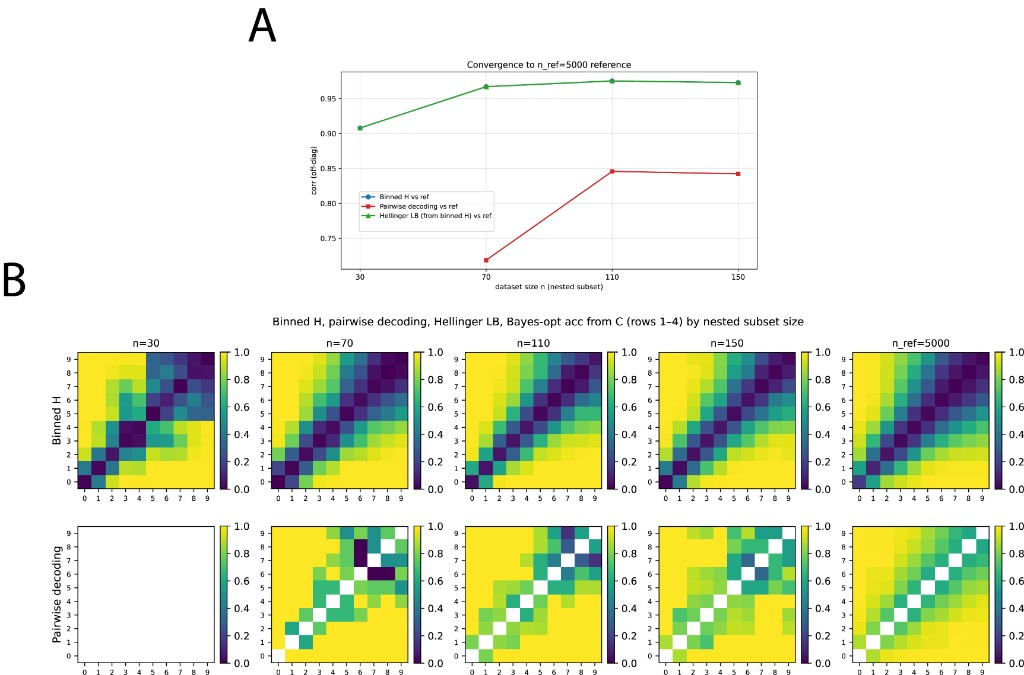
\includegraphics[width=0.7\linewidth]{notes/figures/rsa_nested_subset_convergence.png}
    \caption{Estimation from subset of dataset convergence of geometry estimates to a large reference ($n_{\mathrm{ref}}=5000$). \textbf{(A)}~Correlation of off-diagonal matrix entries to the reference for binned Hellinger ($H$), pairwise decoding, and a Hellinger lower bound derived from binned $H$ (blue and green overlap), as nested subset size $n$ increases. \textbf{(B)}~Heatmaps of binned $H$, pairwise decoding, Hellinger lower bound, and Bayes-optimal accuracy (rows) across $n\in\{30,70,110,150\}$ and the reference column. Pairwise decoding was computed by binning the data and using logistic regression to estimate decoding accuracy. Dataset: linear tuning $(x,2x)$ with Gaussian noise std linearly ramped from 0.2 to 4.}
    \label{fig:rsa_nested_subset_convergence}
\end{figure}
\FloatBarrier

\subsection{Supplementary information: From dataset \texorpdfstring{$\{(\theta_i,x_i)\}_{i=1}^N$}{(theta_i,x_i)} to the \texorpdfstring{$h$}{h}-matrix}

We start from a dataset
\[
\mathcal D=\{(\theta_i,x_i)\}_{i=1}^N,
\]
where \(\theta_i\in\mathbb R\) is a scalar condition and \(x_i\) is the corresponding observation. Our goal is to construct an \(N\times N\) matrix
\[
\mathbf H^2=[H_{ij}^2],
\]
whose entry \(H_{ij}^2\) is the sample-wise symmetric contribution of \(x_i\) when comparing the conditional distributions \(p(x\mid \theta_i)\) and \(p(x\mid \theta_j)\).

\paragraph{Step 1: learn posterior and prior scores in \(\theta\).}
Using denoising score matching, we train two score models:
\[
s_{\phi}(\tilde\theta,x,\sigma)\approx \partial_\theta \log p_{\sigma}(\tilde\theta\mid x),
\qquad
r_{\psi}(\tilde\theta,\sigma)\approx \partial_\theta \log p_{\sigma}(\tilde\theta),
\]
where \(p_{\sigma}\) denotes the distribution smoothed in \(\theta\) by Gaussian noise of scale \(\sigma\). Concretely, the posterior score model is trained by minimizing
\[
\mathcal L_{\mathrm{post}}(\phi)
=
\mathbb E_{(\theta,x)\sim \mathcal D,\;\sigma,\;z\sim\mathcal N(0,1)}
\Big[
\big\|
\sigma s_{\phi}(\theta+\sigma z,x,\sigma)+z
\big\|^2
\Big],
\]
and the prior score model is trained by minimizing
\[
\mathcal L_{\mathrm{prior}}(\psi)
=
\mathbb E_{\theta\sim\{\theta_i\},\;\sigma,\;z\sim\mathcal N(0,1)}
\Big[
\big\|
\sigma r_{\psi}(\theta+\sigma z,\sigma)+z
\big\|^2
\Big].
\]

For a small evaluation noise level \(\sigma_{\mathrm{eval}}\), define the recovered Fisher score
\[
\hat g(\theta,x)
:=
s_{\phi}(\theta,x,\sigma_{\mathrm{eval}})
-
r_{\psi}(\theta,\sigma_{\mathrm{eval}}).
\]
By Bayes' rule,
\[
\partial_\theta \log p(x\mid \theta)
=
\partial_\theta \log p(\theta\mid x)-\partial_\theta \log p(\theta),
\]
so \(\hat g(\theta,x)\) approximates the Fisher score \(\partial_\theta \log p(x\mid \theta)\).

\paragraph{Step 2: sort the dataset by \(\theta\).}
For notational simplicity, we assume the samples are reordered such that
\[
\theta_1\le \theta_2\le \cdots \le \theta_N.
\]
If the original dataset is not sorted, we sort it by \(\theta\), perform all computations below in the sorted order, and permute the final matrices back to the original order if desired.

\paragraph{Step 3: construct the recovered Fisher score matrix.}
For each sample \(x_i\) and each observed condition \(\theta_k\), define
\[
G_{ik}:=\hat g(\theta_k,x_i).
\]
Thus \(\mathbf G=[G_{ik}]\in\mathbb R^{N\times N}\) is the matrix whose \(i\)-th row corresponds to a fixed observation \(x_i\), and whose \(k\)-th column evaluates the recovered Fisher score at condition \(\theta_k\).

\paragraph{Step 4: construct the cumulative integral matrix.}
For each row \(i\), define the cumulative trapezoidal integral
\[
C_{i1}=0,
\qquad
C_{i,k+1}
=
C_{ik}
+
\frac{\theta_{k+1}-\theta_k}{2}\bigl(G_{ik}+G_{i,k+1}\bigr),
\quad k=1,\dots,N-1.
\]
Equivalently,
\[
C_{ij}
=
\sum_{k=1}^{j-1}
\frac{\theta_{k+1}-\theta_k}{2}\bigl(G_{ik}+G_{i,k+1}\bigr),
\qquad j=1,\dots,N.
\]
For fixed \(i\), \(C_{ij}\) approximates the integral
\[
C_{ij}\approx \int_{\theta_1}^{\theta_j}\hat g(\theta,x_i)\,d\theta.
\]

\paragraph{Step 5: construct the log-likelihood-ratio matrix \(\Delta \mathbf L\).}
For a sample \((\theta_i,x_i)\), define
\[
\Delta \ell_{ij}(x_i)
:=
\log p(x_i\mid \theta_j)-\log p(x_i\mid \theta_i).
\]
Since
\[
\Delta \ell_{ij}(x_i)
=
\int_{\theta_i}^{\theta_j}\partial_\theta \log p(x_i\mid \theta)\,d\theta,
\]
we estimate it by
\[
\Delta L_{ij}:=C_{ij}-C_{ii}.
\]
Thus the matrix \(\Delta \mathbf L=[\Delta L_{ij}]\in\mathbb R^{N\times N}\) is the estimated log-likelihood-ratio matrix, where
\[
\Delta L_{ij}\approx \Delta \ell_{ij}(x_i).
\]
By construction,
\[
\Delta L_{ii}=0.
\]

\paragraph{Step 6: construct the directed sample-wise contribution matrix.}
Define
\[
H^{\rightarrow}_{ij}
:=
1-\operatorname{sech}\!\left(\frac{\Delta L_{ij}}{2}\right).
\]
This is a directed matrix, because its \((i,j)\)-entry is evaluated on \(x_i\) only.

\paragraph{Step 7: symmetrize the matrix.}
To obtain a symmetric pairwise matrix, average the two directions:
\[
H^{sym}_{ij}
:=
\frac12\left(H^{\rightarrow}_{ij}+H^{\rightarrow}_{ji}\right).
\]
Thus the full pipeline is
\[
\{(\theta_i,x_i)\}_{i=1}^N
\;\longrightarrow\;
s_{\phi},\,r_{\psi}
\;\longrightarrow\;
\mathbf G
\;\longrightarrow\;
\mathbf C
\;\longrightarrow\;
\Delta \mathbf L
\;\longrightarrow\;
\mathbf H^{\rightarrow}
\;\longrightarrow\;
\mathbf H^{sym}.
\]

\paragraph{Algorithmic summary.}
\begin{enumerate}
    \item Train \(s_{\phi}(\theta,x,\sigma)\) and \(r_{\psi}(\theta,\sigma)\).
    \item Compute
    \[
    G_{ik}=s_{\phi}(\theta_k,x_i,\sigma_{\mathrm{eval}})
    -
    r_{\psi}(\theta_k,\sigma_{\mathrm{eval}})
    \]
    for all \(i,k\).
    \item Compute the cumulative integral matrix \(\mathbf C\) row by row:
    \[
    C_{i1}=0,\qquad
    C_{i,k+1}=C_{ik}+\frac{\theta_{k+1}-\theta_k}{2}(G_{ik}+G_{i,k+1}).
    \]
    \item Compute the directed log-ratio matrix
    \[
    \Delta L_{ij}=C_{ij}-C_{ii}.
    \]
    \item Compute the directed contribution matrix
    \[
    H^{\rightarrow}_{ij}
    =
    1-\operatorname{sech}\!\left(\frac{\Delta L_{ij}}{2}\right).
    \]
    \item Symmetrize:
    \[
    H^{sym}_{ij}
    =
    \frac12\left(H^{\rightarrow}_{ij}+H^{\rightarrow}_{ji}\right).
    \]
\end{enumerate}

Finally, the Hellinger distance matrix is given by the expectation which can be computed by binning $H^{sym}_{ij}$ or regression method:
\[
\mathbf H^2=[\mathbb E_{x_i\sim p_i,\;x_j\sim p_j}[H^{sym}_{ij}]].
\]

\subsection{Supplementary information: Hellinger distance and bounds on classification accuracy}

For binary classification between conditions \(i\) and \(j\) with equal class priors, let
\[
p_i(x)=p(x\mid \theta_i),\qquad p_j(x)=p(x\mid \theta_j),
\]
and let \(H_{ij}\) denote the Hellinger distance between \(p_i\) and \(p_j\). The Bayes-optimal classification accuracy is
\[
A^*_{ij}=\frac12\bigl(1+\mathrm{TV}(p_i,p_j)\bigr),
\]
where \(\mathrm{TV}(p_i,p_j)\) is the total variation distance. Using the inequalities
\[
H_{ij}^2 \le \mathrm{TV}(p_i,p_j)\le \sqrt{2H_{ij}^2-H_{ij}^4},
\]
we obtain
\[
\frac12(1+H_{ij}^2)
\le
A^*_{ij}
\le
\frac12\left(1+\sqrt{2H_{ij}^2-H_{ij}^4}\right).
\]
Therefore, a measured Hellinger distance directly constrains the best achievable pairwise classification accuracy. In particular, larger Hellinger distance implies better possible discriminability, with \(H_{ij}=0\) corresponding to chance-level accuracy \(A^*_{ij}=1/2\), and \(H_{ij}=1\) corresponding to perfect classification \(A^*_{ij}=1\).